%%%%%%%%%%%%%%%%%%%%%%%%%%%%%%%%%%%%%%%%%%%%%%%%%%%%%%%%%%%%%%%%%%%%%%%%%%%
%% This file is part of the book
%%
%% Algorithmic Graph Theory
%% http://code.google.com/p/graph-theory-algorithms-book/
%%
%% Copyright (C) 2009, 2010 Minh Van Nguyen <nguyenminh2@gmail.com>
%%
%% See the file COPYING for copying conditions.
%%%%%%%%%%%%%%%%%%%%%%%%%%%%%%%%%%%%%%%%%%%%%%%%%%%%%%%%%%%%%%%%%%%%%%%%%%%

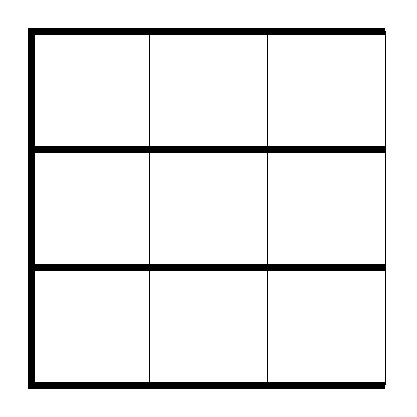
\begin{tikzpicture}
[linedecorate/.style={line width=2.5pt},scale=1.5]
\foreach \x/\ystart/\yend in {1/0/3, 2/0/3, 3/0/3}
{
  \draw (\x,\ystart) -- (\x,\yend);
}
%% draw the spanning tree
\draw[linedecorate] (3,3) -- (0,3) -- (0,0) -- (3,0);
\draw[linedecorate] (0,1) -- (3,1);
\draw[linedecorate] (0,2) -- (3,2);
\end{tikzpicture}
